\chapter[Desenvolvimento e Metodologia]{Desenvolvimento e Metodologia de Testes}

\section{Algoritmo}

\subsection{Seleção de Variáveis \textit{Stepwise}}

O algoritmo proposto nesse trabalho é baseado no método de seleção de variáveis \textit{stepwise} 
(\textit{Stepwise Selection}), comumente utilizado em conjunto com modelos de regressão linear. É um método de \textit{greedy search}, onde, a cada iteração, a variável que apresentar o melhor ganho de performance é adicionada ao conjunto de entradas. 

O modelo é construído incrementalmente até que não haja mais melhora de performance ao acrescentar alguma das variáveis restantes ou não haja mais variáveis para serem consideradas. O método é descrito em pseudocódigo no Algoritmo \ref{alg:stepwiseselection}.

\qquad

\begin{algorithm}[!htb]
    \caption{\textit{Forward Stepwise Selection} (FSS)}
    \KwIn{$variáveis$: lista contendo as variáveis disponíveis;}
    \KwIn{$saídas$: lista contendo as saídas do modelo;}
    \KwOut{$selecionadas$: lista de variáveis relevantes.}
    $selecionadas \gets \{\ \}$ \\
    $melhorErro \gets \infty$ \\
    \Repeat{$variáveis == \{\ \}$ ou (critério de parada)}
    {   
        $melhorVariável \gets NULL$ \\     
        \ForEach{elemento $var$ em $variáveis$}{
            $entradas \gets (var \cup selecionadas)$ \\
            $model \gets ajuste(entradas,saídas)$ \\
            $erro \gets avalia(model,entradas,saídas)$ \\
            \If{$erro <melhorErro$}{
                $melhorErro \gets erro$\\
                $melhorVariável \gets var$ \\     
            }
        }
        $selecionadas \gets (melhorVariável \cup selecionadas)$ \\
        $variáveis \gets (variáveis \setminus \{melhorVariável\})$ \\
    }
    \label{alg:stepwiseselection}
\end{algorithm}

\qquad

No método da seleção do melhor subconjunto, que é um algoritmo de busca exaustiva, todas as combinações possíveis das variáveis de entrada são testadas. No algoritmo \textit{Stepwise} porém, há uma redução expressiva na quantidade de modelos ajustados. Na primeira iteração, o modelo nulo deve ser ajustado, em seguida, todas as $p$ variáveis devem ser avaliadas e, a cada iteração posterior, uma delas é retirada.

Porém, ao contrário do método da seleção do melhor subconjunto, não há garantia que o subconjunto determinado é a combinação ótima das variáveis \cite[p. 208]{intro_stat_learn}.

Um fator determinante para a eficácia do algoritmo é a escolha da métrica pela qual os modelos serão avaliados. A utilização de uma métrica que considere simplesmente os dados ajustados não é adequada, 
uma vez que, nessa situação, o incremento de uma variável no modelo sempre acarretará em uma melhora no erro de treinamento, porém não necessariamente na capacidade de generalização do modelo.

Algumas técnicas tentam determinar a capacidade de generalização através de informações obtidas com os dados de treinamento, tais como o critério de Informação de Akaike (AIC) ou critério de informação Bayesiano (BIC), porém elas se baseiam no comportamento assintótico, isto é, quando a quantidade de amostras é bastante elevada.

Uma alternativa a essas métricas é a utilização de validação cruzada, onde o modelo selecionado é aquele que apresenta a melhor performance no conjunto de testes. Dessa maneira, obtém-se diretamente uma estimativa do erro de generalização, além de se assumir menos condições em relação ao modelo e aos dados utilizados. 

O grande empecilho à implementação de validação cruzada é seu custo computacional que, quando associado ao custo do método de seleção de variáveis \textit{stepwise}, pode tornar proibitiva sua implementação.

Em especial, a utilização desse método associada ao \textit{leave-one-out cross-validation} resultaria no ajuste de um número significativamente elevado de modelos, tornando o algoritmo computacionalmente inviável.
\FloatBarrier

\subsection{Método Incremental}

Para minimizar o problema do custo computacional, o método implementado utiliza o resultado apresentado na eq. \ref{eq:LOOCV_error} para calcular o erro de validação cruzada sem a necessidade de calcular $N-1$ modelos de regressão linear. Além disso, o cálculo da matriz de aniquilação é realizado de maneira incremental, conforme deduzido na eq. \ref{eq:inc_matrix_iterativa}.

O Algoritmo \ref{alg:stepwiseselection} é então modificado no Algoritmo \ref{alg:incstepwiseselection} para realizar o cálculo incremental, utilizando LOOCV como métrica para seleção das variáveis e atualização incremental do modelo.

\begin{algorithm}[!htb]
    \caption{\textit{Forward Stepwise Incremental Selection}}
    \KwIn{$variáveis$: lista contendo as variáveis disponíveis;}
    \KwIn{$saídas$: lista contendo as saídas do modelo;}
    \KwOut{$selecionadas$: lista de variáveis relevantes.}
    
    $selecionadas \gets \{\ \}$ \\
    $melhorErro \gets \infty$ \\
    $M \gets I_N$ \\

    \Repeat{$variáveis == \{\ \}$ ou (critério de parada)}
    { 
        $melhorVariável \gets NULL$ \\
        \ForEach{elemento $var$ em $variáveis$}{
            $M' \gets ajusteIncremental(M,var)$ \\
            $erro  \gets erroLOOCV(M,saídas)$ \\
            \If{$erro <melhorErro$}{
                $melhorErro \gets erro$\\
                $melhorVariável \gets var$ \\                
                $melhorM \gets M' $  \\
            }
        }
        $M \gets melhorM $ \\
        $selecionadas \gets (melhorVariável \cup selecionadas)$ \\
        $variáveis \gets (variáveis \setminus \{melhor_{variável}\})$ \\
    }
    \label{alg:incstepwiseselection}
\end{algorithm}

O código em R que implementa o algoritmo proposto se encontra no Apêndice \ref{appendix:step_wise_code} desse trabalho.

\FloatBarrier
\subsection{Complexidade algorítmica}

A implementação não incremental do método \textit{stepwise} resulta no ajuste de uma curva para cada conjunto de variáveis considerado. Como apenas uma variável é acrescentada a cada etapa, o total de modelos ajustados pode então ser derivado como na eq. \ref{eq:naive_stepwise}.

\begin{equation}
    1 + \sum^{p-1}_{k=0} (p-k) = 1+p(p+1) = \frac{1}{2}(p^2+p+2)
    \label{eq:naive_stepwise} 
\end{equation}

Quando associado ao cálculo do erro de validação cruzada \textit{leave-one-out}, para cada conjunto de varáveis considerado, é necessário o cálculo de $(N-1)$ modelos, cada um excluindo uma amostra do treinamento. Dessa forma a equação eq. \ref{eq:naive_stepwise} deve ser multiplicada por esse fator.

Analisando a eq. \ref{eq:lsnormal_reg}, é possível assumir a complexidade de uma implementação simples do ajuste de uma regressão linear como $\bigO{Np^2 + p^3}$. Implementações utilizando algoritmos otimizados de multiplicação e inversão de matrizes podem reduzir essa complexidade. A custo de uma predição pode ser facilmente percebido como $O(p)$.

Sendo assim, a complexidade da implementação não incremental do método \textit{stepwise} pode ser derivada conforme a eq. \ref{eq:naive_stepwise_loocv}.
\begin{equation}
    \begin{split}
        O(Stepwise_{LOOCV}) &= \frac{1}{2}(p^2+p+2)(N-1)\left( \bigO{Np^2 + p^3}+\bigO{p}\right) \\
                            &= \bigO{p^2}\ \bigO{N}\ \bigO{Np^2 + p^3} \\
                            &= \bigO{N^2p^4 + Np^5}
    \end{split}
    \label{eq:naive_stepwise_loocv}
\end{equation}

O método proposto neste trabalho não realiza o ajuste direto do modelo, mas sim o cálculo de maneira incremental da matriz de aniquilação. Dessa forma, além de não ser necessário o cálculo da inversão da matriz $A$ na eq. \ref{eq:lsnormal_reg}, o cálculo do erro de validação cruzada \textit{leave-one-out} pode ser calculado diretamente, sem a necessidade de $N-1$ passos. Dessa maneira o custo computacional é reduzido para o exposto na eq. \ref{eq:inc_stepwise_loocv}.
\begin{equation}
    \begin{split}
        O(Stepwise_{LOOCV}^{INC}) &= \frac{1}{2}(p^2+p+2)\left( \bigO{3 N^2}\right)\\
                            &= \bigO{p^2}\ \bigO{N^2} \\
                            &= \bigO{N^2p^2}
    \end{split}
    \label{eq:inc_stepwise_loocv}
\end{equation}

\section{Testes}

\subsection{Conjuntos de dados}

Para teste do algoritmo desenvolvido, utilizou-se quatro bancos de dados conhecidos na literatura, 
especificados na tabela \ref{tbl:datasets}.
\begin{table}[H]
    \caption{Conjuntos de dados utilizados para teste.}
    \centering
    \begin{tabular}{@{}lll@{}}
    \toprule
    Nome                           & Variáveis & Amostras \\ \midrule
    \textit{Communities and Crime} \cite{ds_crime} & 101       & 2215     \\
    \textit{Forest Fires} \cite{ds_forest}         & 12        & 517      \\
    \textit{USA Housing Dataset} \cite{ds_house}   & 80        & 1460     \\
    \textit{Wiscoin Breast Cancer} \cite{ds_cancer}& 32        & 194      \\ \bottomrule
    \end{tabular}
    \label{tbl:datasets}
\end{table}

\subsubsection{Pré-processamento}

De maneira geral, em um conjunto de amostras, as variáveis apresentam diferentes unidades, magnitudes e escalas. Tal variação dificulta a comparação de valores e pode prejudicar o treinamento de modelos. Por isso é comum aplicar uma transformação nos dados, de maneira a torná-los comparáveis entre si (\textit{feature scaling}), além de facilitar a detecção de \textit{outliers}.

Embora o algoritmo utilizado se baseie em regressões lineares que, em sua forma mais simples, são robustas em  relação a magnitude das variáveis, a adição do termo de regressão penaliza o crescimento do vetor de parâmetros, tornando o modelo sensível à diferença de magnitudes entre variáveis.

Neste trabalho, todas as variáveis foram normalizadas, de maneira a se obter entradas e saídas que apresentam média nula e desvio padrão unitário. Tal transformação é conhecida como \textit{z-score} (eq. \ref{eq:z-score}).

\begin{equation}
    X_p = \frac{ X_p - \bar{X_p} }{SD(X_p)}
    \label{eq:z-score}
\end{equation}

Além disso, uma variável de entrada com valor unitário foi adicionada posteriormente a cada conjunto de dados, permitindo a consideração do termo livre ($w_0$) nos cálculos de maneira transparente.

\subsection{Metodologia de Teste}

Com o intuito de identificar um subconjunto ótimo de variáveis para cada conjunto de dados, o algoritmo 
desenvolvido foi empregado e o erro de validação cruzada, conforme a eq. \ref{eq:LOOCV_error}, foi registrado ao final de cada iteração. Dessa maneira, é possível analisar o efeito da inclusão de uma nova variável na capacidade de generalização do modelo e avaliar o quão benéfico é o aumento de uma nova dimensão.

Em seguida, para cada conjunto de dados, dois modelos são treinados com parâmetros idênticos, variando-se o conjunto de variáveis. Dessa maneira, é possível estudar quais os efeitos da utilização do subconjunto proposto pelo algoritmo em relação ao conjunto completo de variáveis.

Optou-se pela utilização de um modelo \textit{Perceptron} (MLP) de uma camada oculta (três camadas no total: entradas, camada oculta, saída), devido a disponibilidade de implementações disponíveis tanto para o modelo, quanto para o seu treinamento e validação.

Utilizou-se a biblioteca Keras \cite{keras} com a interface para a linguagem R e a biblioteca Tensorflow \cite{tensorflow} como \textit{backend}. O código fonte que implementa a rede neural desenvolvida se encontra no Apêndice \ref{appendix:keras_mlp}.

% \section{Estudo de Caso: Vallourec - Caracterização de tubos de aço}

% \subsection{Descrição do Problema}

% Para que um tubo possa ser utilizado na extração de petróleo e gás, ele deve ser submetido a diversos testes e receber uma certificação que comprove que o mesmo está adequado para utilização.

% O teste em questão, verifica a resistência à corrosão sob tensão. Durante a sua realização, um corpo de prova extraído do tubo é imerso em uma solução ácida e deve resistir sem fraturas durante 720 horas. Todo o lote de tubos deve aguardar o resultado do teste para ser despachado. Caso 2 corpos de prova falhem, o material deve ser retratado e o teste refeito. 

% \begin{figure}
%     \caption{Estruturas de teste}
%     \begin{subfigure}{.5\textwidth}
%       \centering
%       \includegraphics[width=.8\linewidth]{imgs/met/corpo_de_prova}
%       \caption{Corpo de prova utilizado para o teste}
%       \label{fig:corpo_de_prova}
%     \end{subfigure}%
%     \begin{subfigure}{.5\textwidth}
%       \centering
%       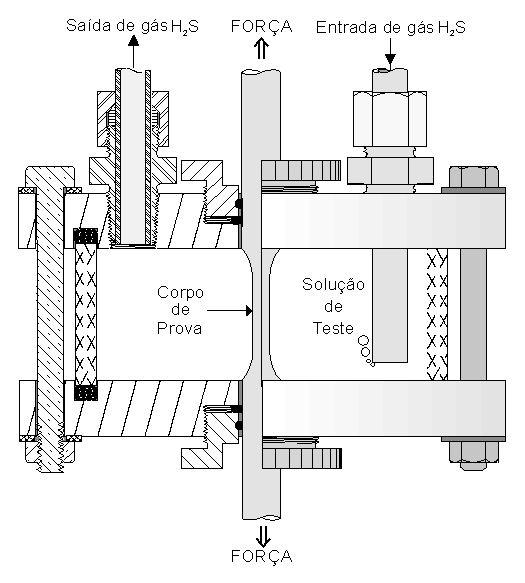
\includegraphics[width=.8\linewidth]{imgs/met/estrutura_de_teste}
%       \caption{Esquemático da câmara para a realização do teste}
%       \label{fig:sfig2}
%     \end{subfigure}
%     \legend{Fonte: NACE Standard TM0177 \cite[p. 7,8]{nace_standart} (Adaptada)}
%     \label{fig:estrutura_de_teste}
%     \end{figure}

% O grande tempo despendido durante o teste e a necessidade de aguardar o resultado para prosseguir para as etapas seguintes de produção resulta em aumento de estoques e altos tempos para o atendimento dos pedidos dos clientes (lead time).

% Diversas características que podem influenciar no resultado do teste foram levantadas e objetiva-se a determinação daquelas com maior significância para a determinação de um modelo capaz de realizar predições do resultado do teste.

% \subsection{Descrição do Conjunto de dados}

% Utilizando-se o conhecimento prévio do processo, uma filtragem inicial dos dados foi realizada, removendo caracteristicas irrelevantes para o processo de modelagem, tais como identificações, lotes e datas. Variáveis que não apresentam nenhuma variação no conjunto de dados também foram removidas. Além disso, por motivos de confidencialidade, o nome das variáveis foram anonimizados. Por fim, os dados passaram pelo processo de normalização descrito anteriormente.

% Após o processamento inicial, o conjunto de dados possui 1064 amostras, com 30 possíveis variáveis de entrada e 3 varíaveis de saída.

% \subsection{Metodologia}

% O objetivo principal nesse estudo é identificar qual o melhor subconjunto de variáveis para descrever o problema. Por isso, o algoritmo proposto foi executado nesse banco de dados e a curva de performance dos subconjuntos levantada. 

% Quatro modelos foram treinados, sendo dois utilizando o conjunto total de variáveis e dois utilizando o melhor subconjunto sugerido pelo método de seleção. Antecipa-se uma melhora de desempenho ao utilizar um conjunto reduzido de variáveis.

% De maneira auxiliar, a correlação linear entre variáveis e a correlação entre saídas e variáveis foi levantada, de maneira a observar se através dessas medidas é possível identificar uma relação com o subconjunto proposto.
